%%%%%%%%%%%%%%%%%%%%%%%%%%%%%%%%%%%%%%%%%%%%%%%%%%%%%%%%%%%%%%%%%%%%%%%%%%%%%%%%%%%%%%%%%%%%
%%
%% Chapter 5 : Current progress
%%
%%      * Should describe the current state we are in the implementations, research, etc.
%%
%%%%%%%%%%%%%%%%%%%%%%%%%%%%%%%%%%%%%%%%%%%%%%%%%%%%%%%%%%%%%%%%%%%%%%%%%%%%%%%%%%%%%%%%%%%%

\chapter{Current progress}
\label{ch:current_progress}

%%%%%%%%%%%%%%%%%%%%%%%%%%%%%%%
%   Figures for chapter 5
%%%%%%%%%%%%%%%%%%%%%%%%%%%%%%%

\newcommand{\figProgressAgents}{
    \begin{figure}
        \centering
        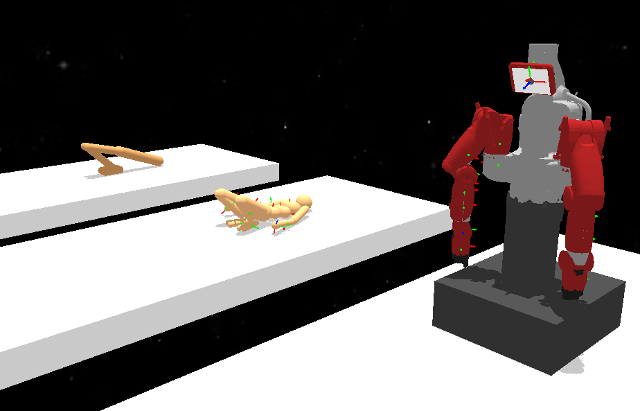
\includegraphics[width=0.9\textwidth]{./chapters/chapter_5/imgs/img_tysocmjc_agents.png}
        \caption{Current agent support. Currently the framework support mjcf
                 formats (from the mujoco engine)}
        \label{fig:ch5_progress_agents}
    \end{figure}
}

\newcommand{\figProgressSensors}{
    \begin{figure}
        \centering
        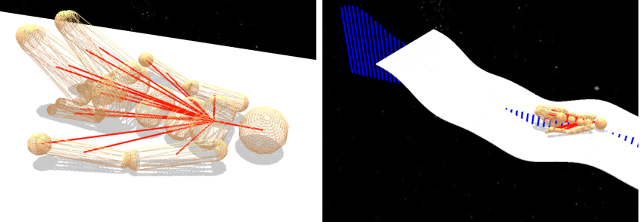
\includegraphics[width=0.9\textwidth]{./chapters/chapter_5/imgs/img_tysocmjc_sensors.png}
        \caption{Current sensor support. Currently the framework supports: 
                            a) intrinsic measurements (joint angles and velocities, body velocities and acceelrations, and relative positions).
                            b) extrinsic measurements (height fields taken from the terrain)}
        \label{fig:ch5_progress_sensors}
    \end{figure}
}

\newcommand{\figProgressTerrains}{
    \begin{figure}
        \centering
        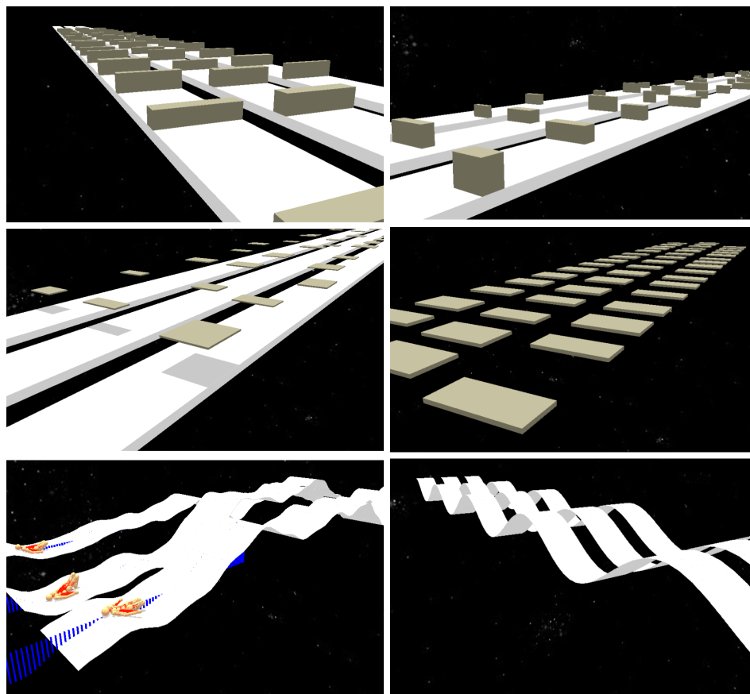
\includegraphics[width=0.9\textwidth]{./chapters/chapter_5/imgs/img_tysocmjc_terrains.png}
        \caption{Current terrain support. Currently the framework supports the
                 environments from \citeauthor{DeepmindEmergenceLocomotion}}
        \label{fig:ch5_progress_terrain}
    \end{figure}
}

In this chapter we discuss the current progress of the proposed framework. The implementation
is still not in version 0.1, which should be the first fully functional version to be released
according to the features proposed in the previous chapter. Nevertheless, the core implementation
needed for the multi-engine support and all other features is at a 70 percent, \todo{Creo que debes colocar porcentajes, como demuestras que estas en un 70 y no 60?}
with the remaining
30 percent corresponding to some additional core features, some bugs, issues, small cleanup and 
documentation of the core functionality. We split the current discussion into the three main 
components that have been implemented so far: core agents support, core sensors support, core 
terrain support, and other utilities.

\section{Agents support}

The implementation of the agent's core functionality has been completed to a 80\%,
remaining only an additional implementation of the agents format provided by \cite{TerrainRLSim}.
This implementation includes the agent's kinematic tree implementation and the integration 
with the MuJoCo physics engine via an adapter written for this specific engine.

The core implementation remains agnostic of the specific engine, which allows us
to make support quickly for the remaining proposed physics engines via adapter code
written once for each platform. The current supported agents are shown in Figure ~\ref{fig:ch5_progress_agents},
which basically shows the support for agents made for MuJoCo via its XML representation format.

The current implementation can be already used for experiments from C/C++. The exposed
functionality includes the supported functionality exposed by most benchmarks, which
give access to the actions via torques. The remaining part of the implementation of the core
agent functionality should give more support for different types of actuation models, like in \cite{ActuationChoice}.

\figProgressAgents

\section{Sensors support}

The implementation of the sensors' core functionality is completed to a 70\%,
remaining some sensors for more complicated tasks: visual inputs from a fixed camera,
and heightmap measurements from more complicated terrains. The current supported sensor
features shown in Figure ~\ref{fig:ch5_progress_sensors}, and consist of:

\begin{itemize}
    \item Intrinsic sensor measurements, like joints angles and velocities, bodies velocities
          and accelerations, and bodies relative positions (to the root body).
    \item Extrinsic sensor measurements, which consist on heightfield data from the terrain ahead,
          taken with respect to the root body.
\end{itemize}

\figProgressSensors

\section{Terrain support}

The current implementation of the core terrain functionality supports procedurally generated
terrain, similar to \cite{DeepmindEmergenceLocomotion}. The core functionality handles 
the creation of primitives from terrain generators, and then this is stored as 
requests for creation in the specific adapters for specific engines. The current 
supported engine is MuJoCo, and we plan in adding full support for more complex 
terrains (and an API to use it), and full support for the remaining proposed physics 
engines. Some screenshots of the current terrain implementations are shown
in Figure ~\ref{fig:ch5_progress_terrain}.

\figProgressTerrains

\todo{deberías cerrar el capítulo con una discusión breve de lo que se hizo}